\documentclass[FM,BP]{tulthesis}
% tento dokument používá balíky specifické pro XeLaTeX a lze jej přeložit
% jen XeLaTeXem, nemáte-li instalována použitá (komerční) písma, změňte
% nebo vymažte příkazy \set...font na následujících řádcích

\newcommand{\verze}{1.10}

\usepackage{polyglossia}
\setdefaultlanguage{czech}
\usepackage{xevlna}

\usepackage{makeidx}
\makeindex

% fonty
\usepackage{fontspec}
\usepackage{xunicode}
\usepackage{xltxtra}
% \setmainfont[Mapping=tex-text,BoldFont={* Bold},Numbers=OldStyle]{Baskerville 10 Pro}
% \setsansfont[Mapping=tex-text,BoldFont={* Bold},Numbers=OldStyle]{Myriad Pro}
% \setmonofont[Scale=MatchLowercase]{Vida Mono 32 Pro}

% příkazy specifické pro tento dokument
\newcommand{\argument}[1]{{\ttfamily\color{\tulcolor}#1}}
\newcommand{\argumentindex}[1]{\argument{#1}\index{#1}}
\newcommand{\prostredi}[1]{\argumentindex{#1}}
\newcommand{\prikazneindex}[1]{\argument{\textbackslash #1}}
\newcommand{\prikaz}[1]{\prikazneindex{#1}\index{#1@\textbackslash #1}}
\newenvironment{myquote}{\begin{list}{}{\setlength\leftmargin\parindent}\item[]}{\end{list}}
\newenvironment{listing}{\begin{myquote}\color{\tulcolor}}{\end{myquote}}
\sloppy

% deklarace pro titulní stránku
\TULtitle{Rozpoznávání emocí v audio nahrávkách s využitím hlubokých neuronových sítí}{}
\TULauthor{Tomáš Petříček}

% pro bakalářské, diplomové a disertační práce
\TULprogramme{B2646}{}{}
\TULbranch{1802T007}{Informační technologie}{Information technology}
\TULsupervisor{Ing. Lukáš Matějů, Ph.D.}
\TULyear{2021}

% Vložil Koprnický, použití bibLateXu
% BibLaTeX settings
\usepackage[ 
backend=biber
%,style=iso-authoryear
,style=iso-numeric
%,style=numeric
%,sortlocale=cs_CZ
,autolang=other
,bibencoding=UTF8
%,urldate=edtf
]{biblatex}
\addbibresource{citations.bib} % vložení seznamu literárních zdrojů v bib formátu / input of references in bib format

%%%%%%%%%%%%%%%%%%%%%%%%%%
% Formátování podle pokynů FZS, čárka mezi jmény a poslední jméno se spojkou „a“
% při volbě iso-authoryear, 
\DeclareDelimFormat{multinamedelim}{\addcomma\space}

\DeclareDelimFormat{finalnamedelim}{%
  \ifnumgreater{\value{liststop}}{2}{\finalandcomma}{}%
  \addspace\bibstring{and}\space}

\DeclareNameAlias{author}{family-given/given-family} 
% kulaté závorky kolem citačního záznamu použitím \parencite{}
% nebo použitím standardního příkazu \cite{} s touto redefinicí \let\cite\parencite
%%%%%%%%%%%%%%%%%%%%%%%%%%

% Hranaté závorky kolem čísel v seznamu literatury při použitém iso-numeric
\DeclareFieldFormat{labelnumberwidth}{\mkbibbrackets{#1}}

\usepackage{csquotes} %užití biblatexu hlasí warnings, důvodem může být použití českých uvozovek v citacích! / solving of problems with Czech quotations
\urlstyle{same} %sazba url odkazů stejným fontem jako ostatní text, řešení problémů v zalamování hypertextových odkazů v citacích / url in references seting into the same form as text 

\begin{document}

\ThesisStart{male}
%\ThesisStart{zadani-a-prohlaseni.pdf}

\begin{abstractCZ}
\end{abstractCZ}

\begin{keywordsCZ}
\end{keywordsCZ}

\vspace{2cm}

\begin{abstractEN}
\end{abstractEN}

\begin{keywordsEN}
\end{keywordsEN}

\clearpage

\begin{acknowledgement}
\end{acknowledgement}

\tableofcontents

\clearpage

\begin{abbrList}
\end{abbrList}

\chapter{Úvod}
Mluvení je nám nejpřirozenější forma komunikace a emoce nám pomáhají si lépe porozumět. Díky emocím můžeme svému okolí ukázat svůj vnitřní psychologický stav. Při používání jiných forem komunikace je těžší vyjádřit své emoce, přesto lidé našli způsoby, jak je do komunikace zapojit. S rozvojem chatovácích platforem byly vyvinuty smajlíky, které reprezentují zjednodušený výraz lidského obličeje. Můžeme, tak ve zprávě poslat úplnější informaci a lépe si porozumět \cite{DBLP:journals/speech/AkcayO20}.

Nicméně i přesto, že jsme schopni vyjádřit své emoce, tak to neznamená, že se pochopíme. Emoce jsou subjektivní a každý z nás je může vnímat trochu jinak. Tato vlastnost emocí neusnadňuje ani vývoj systémů pro jejich rozpoznávání. Zatím nebyl vyvinut způsob, jak emoce měřit. Proto lidé usilují o vyvinutí systémů schopných rozpoznávat emoce bez explicitně zadaných instrukcí.

Modely strojového učení jsou schopné najít skryté vzory v datech a naučit se je rozdělovat. Pro učení modelu pro rozpoznávání emocí lze použít data získaná z textu, změn výrazu tváře, hlasu, gest nebo držení těla \cite{konar_chakraborty_2015}. Modely založené na rozpoznávání emocí z řeči mohou najít uplatnění na příklad při vývoji virtuálních asistentů. 

V posledních letech došlo k rozvoji osobních virtuálních asistentů jako jsou Siri a Alexa, které jsou používány pro hlasové ovládání elektronických zařízení. Mohou odesílat textové zprávy, přijímat telefonní hovory, přehrávat hudbu nebo vyhledávat ve webovém prohlížeči. Systém schopný rozpoznávat emoce může zlepšit komunikaci s asistentem tak, aby se nám zdála přirozenější \cite{DBLP:journals/corr/abs-1912-10458}.

Dále může model najít uplatnění pro call centra. Data generovaná call centrem mohou posloužit k vývoji automatické obsluhy zákazníků nebo pro optimalizaci práce v call centru. Dispečerovi můžou být, podle emocionálního stavu zákazníka, nabídnuty scénáře podle, kterých je vhodné v dané situaci postupovat. Model může být využit také k vylepšení systémů doporučující videa nebo podcasty. Uplatnění může najít také při vývoji realističtějších her. Zdroje dat jsou různé, v dnešní době převažují uměle vytvořené datové sady \cite{konar_chakraborty_2015}.

Práce se zabývá aktuálním tématem a výsledky mohou vést k rozšíření systémů vyvíjených Laboratoří počítačového zpracování řeči Speech Lab \cite{speechlab}. Model by se mohl implementovat na příklad do systému pro zpracování a analýzu řeči pro call-centra.

\chapter{Základy rozpoznávání emocí}

\section{Současné poznání}
% Popis přístupů - co se na to používalo, co se používá teď nejlepší úspěchy
% Používané datasety
Přestože existuje mnoho datových sad, tak většina z nich má do 1 hodiny délky a nahrávky jsou namluveny kolem 10 mluvčích. V rozpoznává řečí je typicky potřeba datová sada s několika sty hodin a větší různorodost mluvčích \cite{konar_chakraborty_2015}.

Dále není v rozpoznávání určeno, které emoce rozpoznávat a jestli pro rozpoznávání používat diskrétní nebo prostorový model. Nicméně při použití diskrétního modelu jsou vymezeny takzvané „big N" emoce, mezi než patří na příklad: hněv, strach, smutek nebo radost \cite{konar_chakraborty_2015}.

Bylo provedeno mnoho pokusů pro rozpoznávání za použití různých modelů, datových sad, příznaků na různých jazycích. Parthasarathy a
Tashev porovnali neuronové sítě typu DNNs, RNNs a 1D-CNN na čínských datových sadách. S 1D-CNN dosáhli výsledků 56 \% procent. Kannan Venkataramanan a Haresh Rengaraj Rajamohan provedli několik pokusů na datové sadě RAVDESS. Použili různé příznaky pro rozpoznávání jako MFCC nebo log Mel spektrogramy a vyzkoušeli modely jako různé varianty CNN a HMM. Nejlepší model 2D CNN s globalním average poolingem dosáhl 70 \% na validačních datech a 66 \% testovacích datech při rozpoznávání emocí do 14 kategorií \cite{DBLP:journals/corr/abs-1912-10458}.

\section{Emoce}
V současnosti není zvolena jednotná definice emocí, existuje jich mnoho. Emoce popisují náš vnitřní stav a jejich tvorba je ovlivněna mnoha faktory jako je osobní zkušenost, fyzické, jednací a komunikační reakce. Pro úlohu rozpoznávání emocí je důležité vědět, jak lze emoce rozdělit \cite{DBLP:journals/speech/AkcayO20}.

Emoce můžeme dělit 2 způsoby podle diskrétního modelu nebo prostorového modelu. Diskrétní model rozšiřuje emoce do kategorií. Mezi hlavní kategorie patří: smutek, radost, strach, hněv, znechucení a překvapení. Prostorový model dělí emoce do jednotlivých prostorů jako jsou mocenství, vzrušení nebo vliv. Vzrušení udává sílu emoce a má rozsah od znudění k nadšení. Výhodou diskrétního modelu je, že je na rozdíl od prostorového modelu intuitivnější. \cite{DBLP:journals/speech/AkcayO20}

\chapter{Datové sady}
K rozpoznávání emocí se používají datové sady, které musí být anotovány. Datové sady pro rozpoznávání emocí jsou děleny do tří hlavních kategorií podle toho, jak byla data získána. Data mohla být pořízena předstíráním, kdy herec při nahrávání předstírá, že emoci prožívá. Tento typ datové sady lze získat spoluprací s profesionálními herci nebo z video záznamů filmů a seriálů. Datovou sadu při spolupráci s herci lze relativně snadno sestavit, protože tvůrci mají poměrně velkou kontrolu nad celým procesem. Tímto způsobem získaná data, ale nemusejí odpovídat reálné situaci, a proto existují další 2 způsoby získávání datových sad. Při získávání vybuzených datových sad je mluvčí umístěn do situace, která se velice podobá reálnému životu. Situace jsou většinou vybírány tak, aby odpovídali potenciálnímu použití \cite{konar_chakraborty_2015}. Poslední způsob získávání dat pro rozpoznávání je z přirozené řeči. Data mohou být získána na příklad z rozhovorů z radií, televizních show nebo záznamů z call center. I přesto, že by tato data měla být pro rozpoznávání nejvhodnější, tak je mnohem obtížnější z nich sestavit datovou sadu. Na data se mohou vztahovat právní nároky a je s nimi více práce při zpracování \cite{DBLP:journals/speech/AkcayO20}.

Datové sady se od sebe mohou lišit také tím, kdo je namluvil. Mluvčí mohou být různého věku a pohlaví a mluvit různými jazyky. Datové sady se také liší tvrzeními, která byla vyslovena. Počet a kategorie rozpoznávacích emocí mohou být také různé \cite{DBLP:journals/speech/AkcayO20}.

Mezi často používané a bezplatné datové sady patří Danish Emotional Speech (DES) database, Berlin Emotional Speech (BES) database, Speech Under Simulated and Actual Stress (SUSAS) database nebo eNTERFACE datová sada \cite{konar_chakraborty_2015}.

\section{Vybrané datové sady}

\subsection{RAVDESS}
Zkratka RAVDESS \cite{Livingstone2018} znamená Ryerson Audio-Visual Database of Emotional Speech and Song a označuje anglickou datovou sadu obsahující nahrávky řeči a písní. Spolu s nahrávkami zvuku byly pořízeny i video záznamy mluvčích. Nahrávky byly namluveny 24 herci, z kterých bylo 12 žen a 12 mužů činící datovou sadu pohlavně vyrovnanou. Mluvčí mluvili severoamerickou angličtinou. Nahrávky řeči zachycují 8 emocí: klid, radost, smutek, hněv, strach, překvapení, znechucení a neutrální stav. Každý herec namluvil 2 tvrzení ve 2 úrovních emocionální intezity, běžnou a silnou, pro všechny emoce. Namluvené výrazy byly „Kids are talking by the door" a „Dogs are sitting by the door". Počet zvukových nahrávek řeči je celkově 1440. Každá nahrávka v datové sadě má přiřazenou anotaci, která udává druh nahrávky, druh emoce, emocionální intezitu, tvrzení, číslo opakování a herce, který nahrávku namluvil. Délky nhrávek se pohybují kolem 3 minut. Datové sada je dostupná buď na webových stránkách smartlaboratory.org nebo na kaggle.com \cite{smart_lab}.

\subsection{SAVEE}
Zkratka SAVEE znamená Surrey Audio-Visual Expressed Emotion a označuje anglickou datovou sadu pro rozpoznávání emocí. Obsahuje 480 promluv a rozlišuje 7 emocí, mezi které patří hněv, znechucení, strach, radost, smutek, překvapení a neutrální stav. Byla namluvena 4 mužskými herci mluvící britskou angličtinou ve věku mezi 27 až 31 lety. Pro tvorbu datové sady bylo vybráno 15 vět z datové sady Texas Instruments a Massachusetts Institute of Technology (TIMIT). Kromě řeči byly při nahrávání zaznamenávány i pohyby v obličeji mluvčích, kteří na něm měli namalovány modré značky \cite{savee}.

\subsection{TESS}
Zkratka TESS \cite{SP2/E8H2MF_2020} znamená Toronto emotional speech set a označuje anglickou datovou sadu pro rozpoznávání emocí. Obsahuje 2800 promluv, které byly namluveny 2 herečkami ve věku 26 a 64 let. Rozlišuje 7 emocí mezi něž patří hněv, znechucení, strach, radost, překvapení, smutek a neutrální stav. Každá herečka namluvila 200 promluv pro všechny emoce. Promluva vždy začínala slovy "Say the word" a končila jedním z 200 vybraných slov \cite{tess}.

\subsection{EMOVO}
EMOVO \cite{DBLP:conf/lrec/CostantiniIPT14} je italská datová sada pro rozpoznávání emocí. Zvukové nahrávky byly vytvořeny 6 herci, z kterých 3 byli muži a 3 ženy. Každý herec vyslovil 14 vět pro každou emoci. Datová sada rozlišuje 7 emocí mezi něž patří znechucení, strach, hněv, radost, překvapení, smutek a neutrální stav \cite{COSTANTINI14.591}.

\section{Předzpracování dat pro rozpoznávání}
Data jsou v typickém systému pro rozpoznávání emocí nejdříve předzpracovány. Z dat jsou nejprve vytaženy příznaky na nízké úrovni. Poté jsou data rozděleny na rámce, z kterých jsou vytaženy příznaky pro rozpoznávání. Dále mohou být na příznaky použity techniky pro snížení počtu příznaků jako je analýza hlavních komponent (PCA) nebo lineární diskriminační analýza (LDA) \cite{konar_chakraborty_2015}.

\subsection{Rámcování}
Rámcování bývá prvním krokem předzpracování dat pro rozpoznávání, kdy je zvukový signál rozdělen na menší časové kousky zvané rámce, které nabývají většinou rozsahu mezi 10-30 milisekundami. Často se jednotlivé rámce překrývají 30 \% až 50 \%, aby se zachoval vztah mezi jednotlivými rámci \cite{DBLP:journals/speech/AkcayO20}. Důvodem rámcování je, že se emoce v průběhu řeči mohou měnit a rozdělení na menší časové úseky zajistí, že se emoce na zůstane v rámci jednoho rámce stejná \cite{konar_chakraborty_2015}.

\subsection{Okénkování}
Po rámcování většinou přichází okénkování, kdy je na jednotlivé rámce použita okénkovácí funkce. Snižuje amplitudu signálu na jeho okrajích a tím snižuje úniky, ke kterým může dojít při použití rychlé Fourierovi transformace (FFT). Pro okénková lze použít Hammingovu okénkovací funkci \cite{DBLP:journals/speech/AkcayO20}.

\subsection{Odstranění ticha}
Dále mohou být použity techniky pro detekci hlasové aktivity. S jejich pomocí může ze signálu odstranit tichá. Mohou být použity metody jako je zero crossing rate, krátkodobá energie nebo autokorelační metody. Metoda zero crossing rate, která udává míru přechodu signálu z kladných do záporných hodnot a naopak v rámci jednoho rámce. Hodnota ukazatele je nízká v místech řeči a vysoká v místech ostatních. Při použití krátkodobé energie dosáhne vysokých hodnot v hlasové části a nízkých hodnotu v částech ostatních. Techniky pro odstranění tichých míst v řeči mohou snížit počet dat a zvýšit jejich přínos pro učení \cite{DBLP:journals/speech/AkcayO20}.

\subsection{Normalizace}
Může být použita také normalizace, která zmírňuje rozdíly v řečí mezi mluvčími a zároveň zachová přenášenou informaci. Normalizace může být použita na více úrovních na úrovni jednotlivých rámců nebo na úrovni celé datové sady. Nejčastěji se pro normalizaci používá z-normalizace \cite{DBLP:journals/speech/AkcayO20}.

\subsection{Odstranění šumu}
Dále mohou být použity techniky na odstranění šumu, který se může během nahrávání do nahrávky dostat. Mezi nejčastěji používané techniky patří nejmenší střední kvadratická chyba (MMSE) a logaritmická spektrální amplituda MMSE \cite{DBLP:journals/speech/AkcayO20}.

\section{Příznaky}
Následuje zvolení vhodných příznaků pro rozpoznávání, kdy jsou z mnoha příznaků vybraný pouze nejvhodnější. Je mnoho příznaků, ale nejsou určeny příznaky, které by se hodili přímo pro rozpoznávání emocí. Ze signálu lze získat jak souhrnné tak lokální příznaky pro rozpoznávání. Mezi souhrnné  příznaky patří na střední hodnota, směrodatná odchylka, minimální nebo maximální hodnota. Lokální příznaky lze získat z jednotlivých rámců a zastupují krátkodobé změny v signálu \cite{DBLP:journals/speech/AkcayO20}.

Příznaky pro rozpoznávání emocí v řeči můžeme dělit na prozodické příznaky, spektrální příznaky, příznaky založené na kvalitě hlasu nebo příznaky založené na Teager Energy Operator (TEO). Nejčastěji používané příznaky při rozpoznávání emocí v řeči jsou prozodické příznaky a spektrální příznaky \cite{DBLP:journals/speech/AkcayO20}.

Mezi prozodické příznaky patří na příklad intonace nebo rytmus. Patří mezi souhrnné příznaky, protože je lze získat z delších hlasových úseků jako jsou hlásky, slova nebo věty. Mezi používané příznaky patří základní frekvence, energie nebo doba trvání. Energie udává míru změny amplitudy signálu v čase. Emoce jako hněv, štěstí nebo překvapení vykazují zvýšenou energii a na druhé straně znechucení a smutek vykazují energii nízkou. Základní frekvence se postupně snižuje při projevení hněvu a naopak stoupá při projevení radosti. Doba trvání potřebná k projevení hněvu je obecně kratší než při projevení smutku \cite{DBLP:journals/speech/AkcayO20}.

Příznaky založené na spektru jsou získávány pomocí Fourierovy transformace, kdy je signál převeden z časové oblasti do oblasti frekvenční a mohou přinést hlubší porozumění signálu než příznaky prozodické. Příznaky jsou získávány z rámců, na které byla použita okénkovací funkce. Příznaky Mel Frequency Cepstral Coefficients (MFCC) jsou založeny na krátkodobém silovém spektru signálu. Mezi další příznaky patří Linear Prediction Cepstral Coefficients(LPCC), Log-Frequency Power Coefficients (LFPC) nebo Gammatone Frequency Cepstral Coefficients (GFCC) \cite{DBLP:journals/speech/AkcayO20}.

Chvění, mihotání nebo poměr harmonie ku hluku (HNR) jsou příznaky založené na kvalitě zvuku. Chvění je měřeno na základě nestálosti frekvence a mihotání je založeno na nestálosti amplitudy. Poměr harmonie ku hluku udává poměr mezi hlukem a frekvenčním spektrem samohlásek \cite{DBLP:journals/speech/AkcayO20}.

Příznaky založené na TEO jsou používány k detekci stresu. Využívají změny svalového napětí, které při stresové situaci nastává. V této kategorii předstihují příznaky jako MFCC a výška tónu.

\subsection{MFCC}
% Příznaky jsou popsány podrobněji, protože jsou používané v praktické části
Technika získávání MFCC příznaků spočívá v okénkování signálu, použití diskrétní Fourierovy transformace, použití Mel banky filtrů, logaritmizace a použití inverzní diskrétní kosínovi transformace. 

Při rámcování je zvukový signál je nejprve rozdělen na jednotlivé posuvné rámce. Dále je signál podroben okénkování, kdy je amplituda signálu snížena na konci a na začátku rámce. Může k tomu být použito Hammingovo nebo Hanningovo okénko. Dále signál převeden pomocí diskrétní Fourierovi transformace do frekvenční oblasti. Na výsledné spektrum aplikujeme Mel banku filtrů, která je založena na Mel stupnici. Mel stupnice zohledňuje vnímaní zvukových frekvencí člověkem. Lidé lépe rozlišují mezi nízkými frekvencemi než mezi vysokými. Dále je signál zlogaritmován a je provedena zpětná Diskrétní kosinová transformace (DCT) \cite{hui_2019}.

\section{Způsoby rozpoznávání emocí}
Pro rozpoznávání emocí se používají klasifikátory nebo regresory, které spadají do oblasti strojového učení s učitelem \cite{DBLP:journals/speech/AkcayO20}. Modely strojové učení s učitelem vyžadují označená data. Každý vzorek musí mít přiřazenou anotaci udávající třídu, do které patří. V případě klasifikace jsou to diskrétní štítky, které odpovídají jednotlivým emocím jako jsou na příklad hněv, radost nebo smutek. V případě regrese jsou to desetinné hodnoty, které označují stupeň mocenství, vzrušení nebo dominance většinou v rozsahu od -1 do +1 \cite{konar_chakraborty_2015}.

Často se při klasifikaci ke vzorku přidávají i vzorky z okolí pro zvýšení kontextu, který může zlepšit výsledky rozpoznávaní. Důvodem je, že emoce ovlivňují dlouhodobé charakteristiky řeči. Přesný počet rámců, který by se měl vzít není určen. Na příklad při použít neuronové sítě typu RNN lze pro zachycení kontextu použít kolem maximálně 10 ramců, jinak model začne trpět problémem mizejícího gradientu. Dalším způsobem, jak klasifikovat emoce je podle statických příznaků jako je maximum, minimum nebo časová délka \cite{konar_chakraborty_2015}.

Při trénování se používá často cross validace, kdy se trénovací a validační sada mění a je vytvořeno několik modelů, kterých výsledky jsou zprůměrovány a je tak dosaženo smysluplnějších výsledkům. U rozpoznávání emocí je používáno především, protože jsou datové sady po většině menšího rozsahu, a tak má rozdělení do jednotlivých sad větší vliv na výsledek. Jako metrika pro ohodnocení modelu se používá přesnost nebo vážená přesnost. Vážená přesnost zohledňuje případný jiný počet vzorků pro každou třídu. Přesnost udává pravděpodobnost, že daný vzorek patří do předpovězené třídy \cite{konar_chakraborty_2015}.

Pro úlohu rozpoznávání emocí v řeči není všeobecně uznaný algoritmus strojového učení, která by se používal. Nicméně nejčastěji používané algoritmy jsou Skryté Markovovy modely (HMM), Gaussian Mixture Model (GMM), Support Vector Machines (SVM), a umělé neuronové sítě (ANN) \cite{DBLP:journals/speech/AkcayO20}.

\chapter{Vybrané základy neuronových sítí}

\subsection{Vícevrstvý perceptron}
Vícevrství perceptron (MLP) neboli feed-forward neural network je složen z více vrstev logických regresí (lineárních vrstev) nasledovanými nelineárními vrstvami. Lineární vrstva se skládá z parametrů vah a biasů a nelineární vrstva se skládá z aktivačních funkcí \cite{DBLP:books/lib/Bishop07}.

Aby mohla být neuronová síť označena za hlubokou neuronovou síť, musí mít 2 a více lineární vrstvy. První vrstva modelu se nazývá vstupní vrstvou a poslední vrstva výstupní vrstvou. Vrstvy mezi vstupní a výstupní vrstvou jsou označovány jako vrstvy skryté. Každá lineární vrstva má svojí šířku, která určuje počet neuronů ve vrstvě. Při klasifikaci do dvou tříd následuje za výstupní vrstvou funkce sigmoid a při klasifikaci do více tříd je funkce softmax.

$$ y_j =  \frac{\mathrm{1} }{\mathrm{1} + e^{-x_j} }  $$ 

Jako aktivační funkce ve skrytých vrstvách jsou pro MLP používány nejčastěji funkce sigmoid a ReLU. jakou Neuronovou síť typu vícevrstvý perceptron lze použít také pro regresy, kdy jsou jako aktivační funkce v nelineárních vrstvách umístěny identity \cite{DBLP:books/lib/Bishop07}.

\subsection{Trénování}
Při trénování neuronové sítě je provedena nejprve dopředná propagace následovaná zpětnou propagací. Po zpětném průchodu sítí jsou parametry sítě upraveny pomocí metody největšího spádu, která minimalizuje ztrátu modelu. Jeden proces učení nazýváme epochou.

Při dopředném průchodu lineární vrstvou jsou vstupní příznaky $ y_i $ přeměněny na výstupní příznaky $ x_j $ pomocí lineární kombinace, kterou lze vyjádřit:

$$ x_j = b_j + \sum_{i}^{N} y_i w_{ij} $$

kde proměnná $ i $ odpovídá indexu příznaku z předchozí vrstvy. $ N $ je celkový počet neuronů předchozí vrstvy. Proměnné $ w_{ij} $ a $ b_j $ reprezentují parametry lineární vrstvy \cite{MATEJU2021327}. Dále jsou příznaky aktivovány nelineární funkcí, kterou lze obecně vyjádřit:

$$ z_j = h(x_j) $$

kde $ x_j $ jsou vstupní příznaky z předchozí vrstvy. Proměnná $ h $ je nelineární, diferencovatelná aktivační funkce a $ z_j $ jsou výstupní příznaky \cite{DBLP:books/lib/Bishop07}.

Proces se opakuje v každé vrstvě sítě. Při dopředném průchodu je nutné si zapamatovat hodnoty vstupních příznaků jednotlivých vrstev sítě, které jsou používány při zpětné propagaci. Výsledkem dopředného průchodu jsou předpovězené hodnoty, z kterých lze pomocí kriteriální funkce získat ztrátu.

Při zpětné propagaci se ztráta modelu propaguje zpět sítí pomocí řetízkového pravidla. Po získání všech gradientů sítě se provede optimalizační algoritmus metody největšího spádu, který aktualizuje parametry sítě. Metodu nejvyššího spádu lze vyjádřit:

$$ x_{t+1} = x_t - \alpha \frac{d}{dx}J(x_t) $$

kde proměnná $ x_{t+1} $ je hodnota aktualizovaného parametru sítě a $ x_t $ je hodnota původního parametru sítě. Hodnota gradientu pro parametr x je $ \frac{d}{dx} $. Ztráta parametru $ x_t $ je označena $ J $.

\subsection{Hyperparametry}
Každý model má také své hyperparametry, které se používají ve fázi učení \cite{leonel_2019}. Hyperparametry mohou měnit strukturu modelu, na příklad u hlubokých neuronových sítí to může být počet a šířka skrytých vrstev nebo aktivační funkce ve skryté vrstvě modelu. Další hyperparametry ovlivňují samotné učení mezi ně patří na příklad míra učení, regularizace nebo počet trénovacích epoch. Míra učení udává míru změny parametrů modelu při jejich aktualizaci. Regularizace zabraňuje přeučení.

\subsection{Hodnocení}
Každý model by měl být, co nejobecnější, měl by dosahovat podobných výsledků jak na trénovacích datech tak na jakýkoli jiných. Když model nedostatečně zobecňuje, tak říkáme, že se nedoučuje. Naopak když se model učí v přílišném detailu, tak říkáme, že se přeučuje. Data jsou proto rozdělena na sadu trénovací a testovací. Model je natrénován na sadě trénovací a otestován na sadě testovací. Dobrý model je úspěšný v podobné míře na obou datových sadách. Trénovací sadu lze dále rozdělit také na sadu trénovací a validační. Validační sada se používá při trénování modelu. Na výsledcích této sady můžeme poznat dříve, jestli se model přeučuje nebo naopak, jestli se učí dostatečně. Při testování na testovací nebo validační sadě se parametry modelu nemění.

Další způsob, jak ohodnotit model, jsou různé metriky. Důležitá metrika, která se používá při hodnocení klasifikátoru, je přesnost udávající poměr mezi správně klasifikovanými vzorky a všemi vzorky. Pro vyhodnocení modelu lze také použít matici záměny, která na jedné ose udává správnou třídu a na druhé předpovězenou třídu. Díky tomu můžeme jednoduše zjistit, jaké třídy si mezi sebou klasifikátor zaměňuje.

% Vybrané koncepty
\subsection{Křížová entropie}
Jako hodnotící kritérium pro klasifikaci do více tříd lze použít křížovou entropii, která měří rozdíl mezi dvěma rozděleními pravděpodobnosti. Lze ji vyjádřit:

$$ l = -{\sum_{c}^{C}t_{c}\log p_{c}} $$

kde $ l $ je výsledná ztráta. Index $ c $ odpovídá klasifikovaným třídám a $ C $ je počet tříd. Proměnná $ p $ značí vstupní pravděpodobnosti pro jednotlivé třídy, které dosahují hodnot od nuly do jedné. $ t $ zastupuje zkutečné třídy. Nabývá hodnoty jedna pro správnou třídu a hodnoty nula pro nesprávnou třídu. Minimalizací křížové entropie minimalizujeme rozdíl mezi pravděpodobnostním rozdělením trénovacích dat a pravděpodobnostním rozdělením předpovídaných hodnot \cite{brownlee_2020}.

\subsection{ReLU}
Rectified linear activation function (ReLU) je aktivační funkce, jejíž výstupem je buď nula, pokud je vstup záporný nebo se hodnota vstupu nezmění, pokud je kladný. Lze ji vyjádřit:

$$ y = max(0, x) $$

kde $ y $ jsou výstupní hodnoty. Proměnná $ x $ zastupuje vstupní hodnoty. Neuronové sítě používající tuto funkci se většinou učí snadněji a dosáhnou lepších výsledků. Výhodou této funkce, je, že nepodléhá přesycení, kdy jsou velká čísla na příklad u funkce sigmoid změněna na 1 a velmi malá čísla 0. Důsledkem přesycení je, že jsou funkce jako sigmoid nebo tanh velice citlivé na hodnoty okolo jejich středu a méně na odlehlejší hodnoty. Následně se to projeví při trénovaná modelu, kdy může dojít k problému mizejícího gradientu u hlubších neuronových sítí \cite{brownlee_2020_ReLU}.

\subsection{Softmax}
Softmax je funkce, která přemění vektor čísel na vektor pravděpodobností, kde jsou pravděpodobnosti pro jednotlivé prvky úměrné velikosti všech prvků vektoru. Funkci lze vyjádřit vzorcem:

$$ p_i = \frac{e^{s_i}}{\sum_{c}^{C}e^{s_c}} $$

kde $ p_i $ je hodnota výstupní pravděpodobnosti. Proměnná $ s $ odpovídá skóre výstupní vrstvy neuronové sítě. Hodnoty $ i $ a $ c $ odpovídají indexu příchozího skóre a $ C $ počtu klasifikovaných tříd. Součet všech výsledných pravděpodobností je roven jedné. Funkce se používá při klasifikaci do více tříd a stojí na konci klasifikátoru. Každá výstupní pravděpodobnost odpovídá jednotlivé třídě datové sady \cite{brownlee_2020_Softmax}.

% používané architektury
% Markovi nepopisovat - nejsou neuronovky
\subsection{Konvoluční neuronové sítě}
Jsou ve velké míře používány pro práci s obrázky. Skládají se z konvolučních vrstev. Každá konvoluční vrstva obsahuje sadu filtrů, jejichž parametry se síť učí \cite{DBLP:journals/corr/abs-1912-10458}.

\subsection{Rekuretní neuronové sítě}
Rekurentní neuronové sítě (RNN) jsou především používány při řešení úloh s daty závislými na čase. Rekurentní neuronové sítě si pamatují skrytý stav, který je vypočítán ze vstupu a vstupuje společně s následujícím vzorkem do sítě. Síť typu RNN je schopna si pamatovat větší kontext a použít ho při předpovídání. Pokročilejším modelem je Long Short-Term Memory (LSTM), který je schopný si poradit s problémem mizejícího a explodujícího gradientu. RNN lze také použít k rozpoznávání emocí, kdy jsou jednotlivé rámce společně s jejich okolí postupně posílány do sítě. Délka rámce s okolím by měla mít alespoň 250 milisekund, aby se byl model schopný naučit rozpoznávat emoce \cite{DBLP:journals/corr/abs-1912-10458}.

\chapter{Vývoj balíčku pro rozpoznávání emocí}
Byl vytvořen balíček s moduly pro rozpoznávání emocí. Balíček je napsán v jazyku Python verze 3. Byly vytvořeny moduly: convertors pro převod dat, data pro práci s daty, classifiers na tvorbu klasifikátoru, files na práci se soubory, datasets k tvorbě datových sad, prepare pro přípravu datových sad a train sloužící k trénování modelu. Modely jsou psány objektově. Byly použity knihivny a frameworky: PyTorch 1.6 pro tvorbu a trénování modelu, seaborn 0.11 a matplotlib 3.3 pro vytvoření grafů, logging 0.4 pro logování při trénování modelu, scikit-learn 0.23 pro rozdělení dat na sety, pandas 1.1 numpy 1.18 pro ukládání a práci s daty, os a sys pro práci s operačním systémem, re pro parsování anotací, subprocess pro spouštění příkazů z příkazové řádky, PyHTK pro načítání souborů vytvořené pomocí sady nástrojů HTK.

\section{Výběr datových sad}
Hlavním kritériem při výběru byla dostupnost datové sady, proto byly vybrány sady bezplatné a dostupné pro vědecké účely. Byly vybrány datové sady především anglické: RAVDESS, TESS a SAVEE a jedna italská: EMOVO. Datové sady mají zastoupení 7 společných emocí, mezi které patří emoce: neutrální, hněv, strach, smutek, spokojenost, odpor a překvapení. Současně mají společně zastoupeny obě pohlaví. Informace o datových sadách byly shrnuty v následující tabulce:

\begin{table}[ht]
\centering
\resizebox{\textwidth}{!}{\begin{tabular}{ccccccc}
  \hline
 název & jazyk & počet tříd & počet mluvčích & pohlaví mluvčích & počet promluv & celková délka (hodiny) \\
  \hline
    RAVDESS & angličtina & 8 & 24 & obě & 1440 & 1.5 \\
    SAVEE   & angličtina & 7 & 4  & muži  & 480  & 0.5 \\
    TESS    & angličtina & 7 & 2  & ženy  & 2800 & 1.6 \\
    EMOVO   & italština  & 7 & 6  & obě & 588  & 0.5 \\
   \hline
\end{tabular}}
\caption{Přehled vybraných datových sad} 
\end{table} 

Celkem tedy byly získány 4 datové sady o 2 jazycích se zastoupením 7 emocí. Dohromady vzniklá datová sada má celkem přibližně dobu trvání 4 hodin.

\section{Předpříprava dat}
Data byla nejdříve předzpracována, byl sjednocen jejich formát a byla převedena na příznaky MFCC. Formát byl sjednocen pomocí nástroje Fast Forward MPEG (FFmpeg) přístupného z příkazové řádky. Nahrávky byly převedeny na vzorkovací frekvenci 16 kHz a byl zachován jeden zvukový kanál. Zvukové nahrávky byly převedeny pomocí příkazu níže:

\begin{figure}[htbp]
\centerline{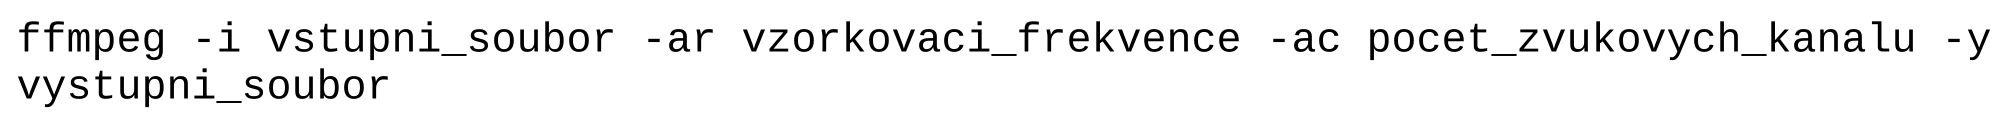
\includegraphics[width=\textwidth,height=\textheight,keepaspectratio]{ffmpeg_command.png}}
\caption{Příkaz FFmpeg}
\label{fig}
\end{figure}

Dále byly nahrávky převedeny na MFCC příznaky. K převodu byl použita sada nástrojů Hidden Markov Model Toolkit (HTK). Pro převod byl použit konfigurační soubor. Převod byl uskutečněn pomocí příkazu:

\begin{figure}[htbp]
\centerline{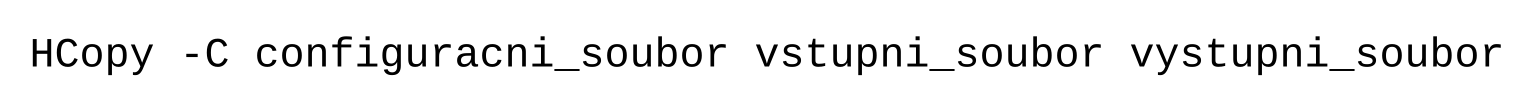
\includegraphics[width=\textwidth,height=\textheight,keepaspectratio]{htk_command.png}}
\caption{Příkaz HTK}
\label{fig}
\end{figure}

Třídy pro převod byly implementovány v modulu conversors. Byla vytvořena základní třída Convertor, z které konkrétní převaděče dědili. Pro sjednocení formátu byla vytvořena třída AudioFormatConverter a třída MFCCConverter pro převod na příznaky MFCC. Vztahy mezi převaděči jsou znázorněni na UML diagramu níže:

\begin{figure}[htbp]
\centerline{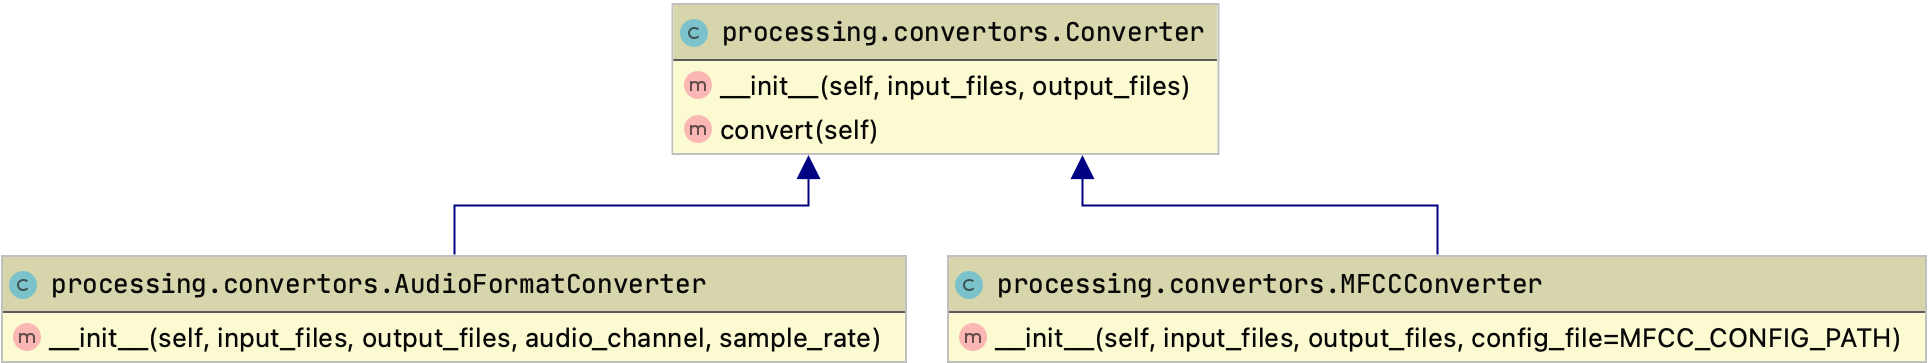
\includegraphics[width=\textwidth,height=\textheight,keepaspectratio]{convertors.png}}
\caption{Třídy Convertor}
\label{fig}
\end{figure}

\section{Příprava datových sad pro trénování}
Pro načítání dat byla vytvořena třída Dataset v modulu data. Hlavními úkoly této třídy bylo načíst data a z anotací získat třídy emocí. Třída Dataset dědí od třídy Directory z modulu files, která umožňuje načíst získat cesty k souborům ve složce. Vztah mezi třídami je znázorněn na diagramu níže:

\begin{figure}[h!]
\centerline{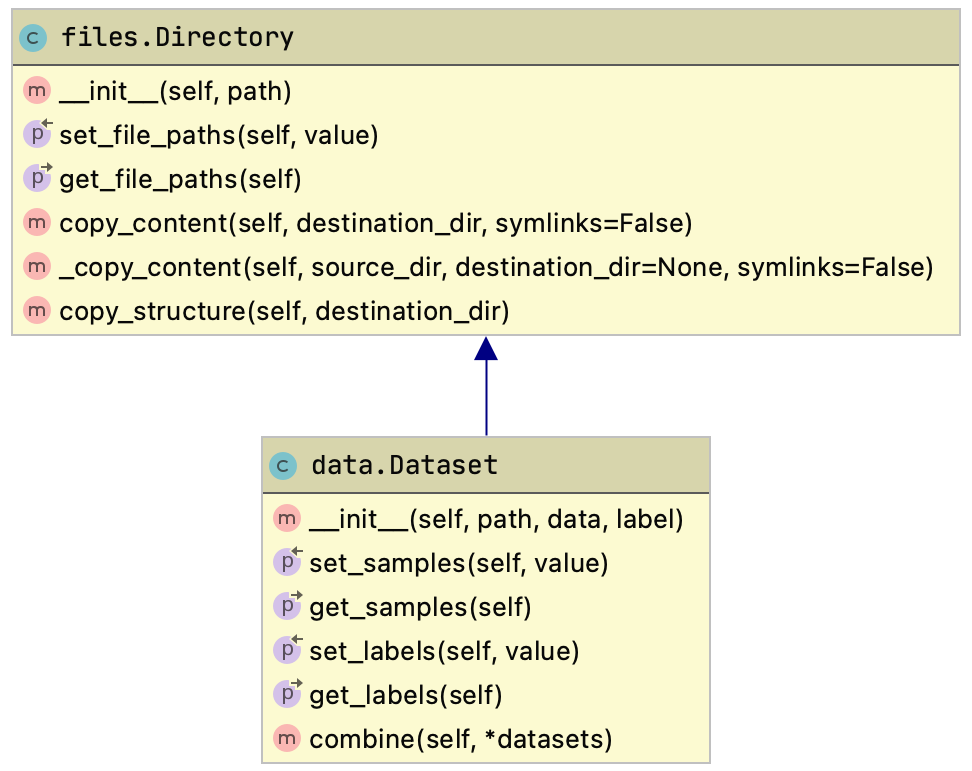
\includegraphics[scale=.25,keepaspectratio]{data-dataset.png}}
\caption{Třída Dataset}
\label{fig}
\end{figure}

Třída Dataset má navíc attributy samples pro uložení načtených vzorků a labels pro uložení anotací pro vzorky. Při vytváření objektu třídy Dataset jsou předávány objekty třídy Data a Label. Objekt třídy Data na základě cesty k souboru načte vzorek a Label z anotace získá informace potřebné k vytvoření anotace pro vzorek. Jelikož jsou datové sady odlišně značeny byly vytvořeny třídy dědící od třídy UnifiedLabel, které navíc anotace pro vzorek převedly na stejné značení. Na následujícím diagramu jsou vidět vztahy mezi třídami Label:

\begin{figure}[h]
\centerline{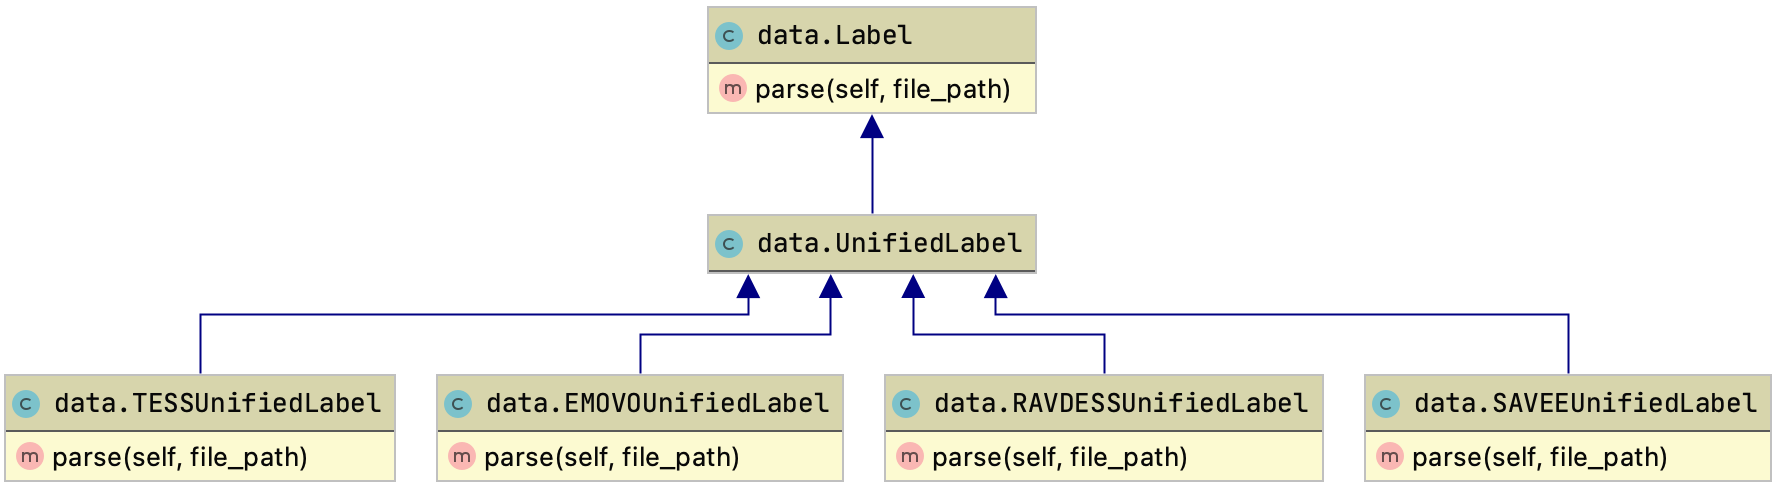
\includegraphics[scale=.25,keepaspectratio]{data-label.png}}
\caption{Třídy Label}
\label{fig}
\end{figure}

Z třídy data dědí třída MFCCData umožňující načtení příznaků MFCC a WAVData zprostředkovávající načtení nahrávek ze souboru typu WAV. MFCCData používá třídu HTKFile z balíčku PyHTK pro načtení příznaků.

\begin{figure}[h]
\centerline{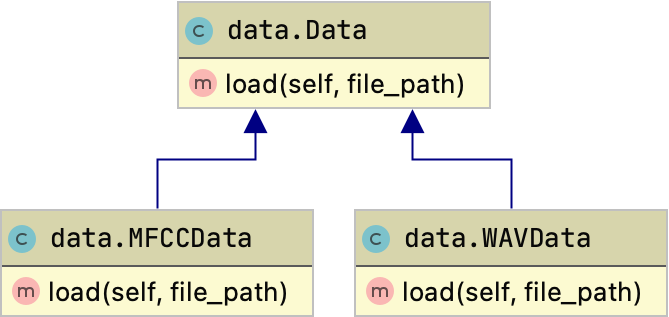
\includegraphics[scale=.25,keepaspectratio]{data-data.png}}
\caption{Třídy Data}
\label{fig}
\end{figure}

Dále byla data rozdělena do trénovacích, validačních a testovacích setů. Pro rozdělení byla použita třída Preparer z modulu prepare. Data byla nejdříve načtena pomocí objektů třídy Dataset. Mohla být sloučena dohromady, na příklad mohla být vytvořena datová sada ze všech anglických datových sad. Data získaná z objektu Dataset mohla být rozdělena do trénovacího, testovacího a validačního setu. Rozdělení probíhalo rovnoměrně třídy train\_test\_split z modulu sklearn.model\_selection a vzorky byly rozděleny po celých nahrávkách. Při rozdělování na sety byla zvolena možnost stratify, která rozdělila vzorky rovnoměrně do vzniklých setů podle anotací.

\begin{figure}[h]
\centerline{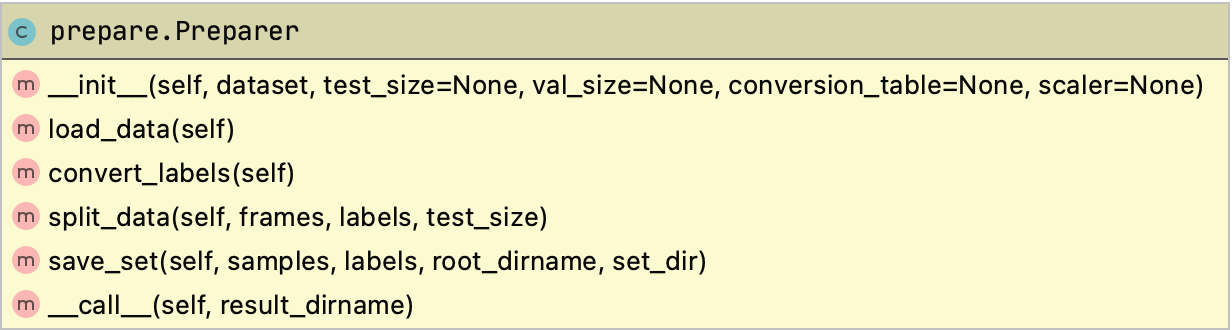
\includegraphics[scale=.25,keepaspectratio]{prepare.png}}
\caption{Třída Preparer}
\label{fig}
\end{figure}

Jako poslední byly sety uloženy do složky. Každému setu byla přiřazena svoje složka, která obsahovala soubory labels.npy, samples.py a info.txt. V souboru info.txt byly uloženy informace pro načítání datového setu. Pro ukládání a načítání informací z ze souborů info.txt byly vytvořeny třídy DatasetInfoFile a SetInfoFile. V souboru třídy DatasetInfoFile byly ulož údaje o počtu příznaků, počtu tříd a počtu vzorků datové sady. Do SetInfoFile byly ukládány počty vzorků, délky vzorků a názvy souborů se vzorky a anotacemi. Data pro rozpoznávání byla uložena ve dvourozměrném poli z balíčku numpy.

\begin{figure}[h]
\centerline{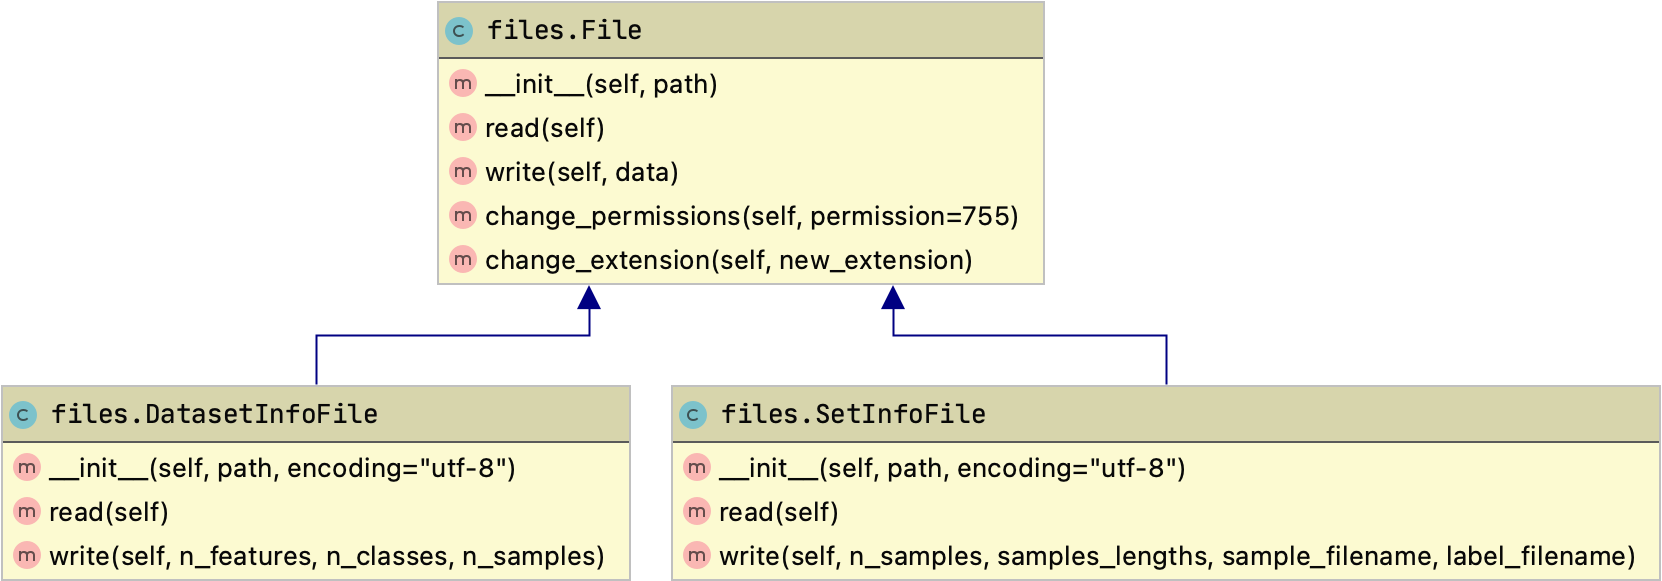
\includegraphics[scale=.25]{files-info.png}}
\caption{Třídy InfoFile}
\label{fig}
\end{figure}

\begin{figure}[h]
\centerline{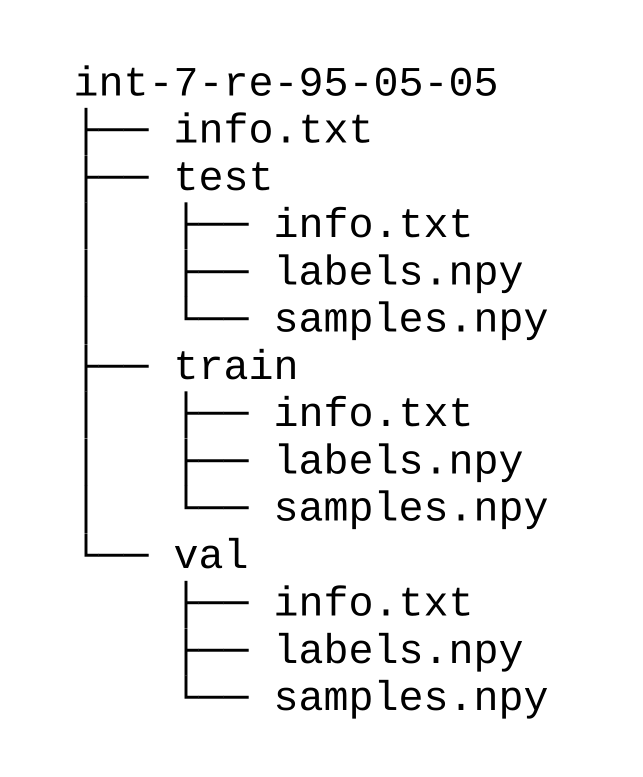
\includegraphics[scale=.2]{dataset_file_structure.png}}
\caption{Souborová struktura uložené datové sady}
\label{fig}
\end{figure}

\section{Načítání dat}
Pro načítání uložených datových sad byl vytvořen objekt NumpyDataset, který dědí od objektu Dataset z balíčku torch.utils.data. Objektu je přidělena cesta k datové sadě. Z textového souboru info.txt si přečte informace potřebné k načtení dat. Mezi důležité parametry, které objekt NumpyDataset při svém vytvoření přebírá jsou velikosti pravé a levého okolí vzorku. Při načtení vzorků ze souboru samples.py jsou ke vzorkům na začátku a na konci přiřazeny okraje, které mají velikosti pravého a levého okolí. Okraje jsou vytvořeny z kopií krajních vzorků a slouží pro zjednodušení výběrů vzorků. Vzorky jsou uloženy popořadě po jednotlivých nahrávkách. Objekt si ukládá indexy začátku a konce nahrávek. Načtené anotace z připravené datové sady odpovídají jednotlivým nahrávkám, proto jsou anotace roztaženy tak, aby odpovídali délce vzorů nahrávky. Uložení vzorků v objektu NumpyDataset je znázorněno na následujícím diagramu:

\begin{figure}[htbp]
\centerline{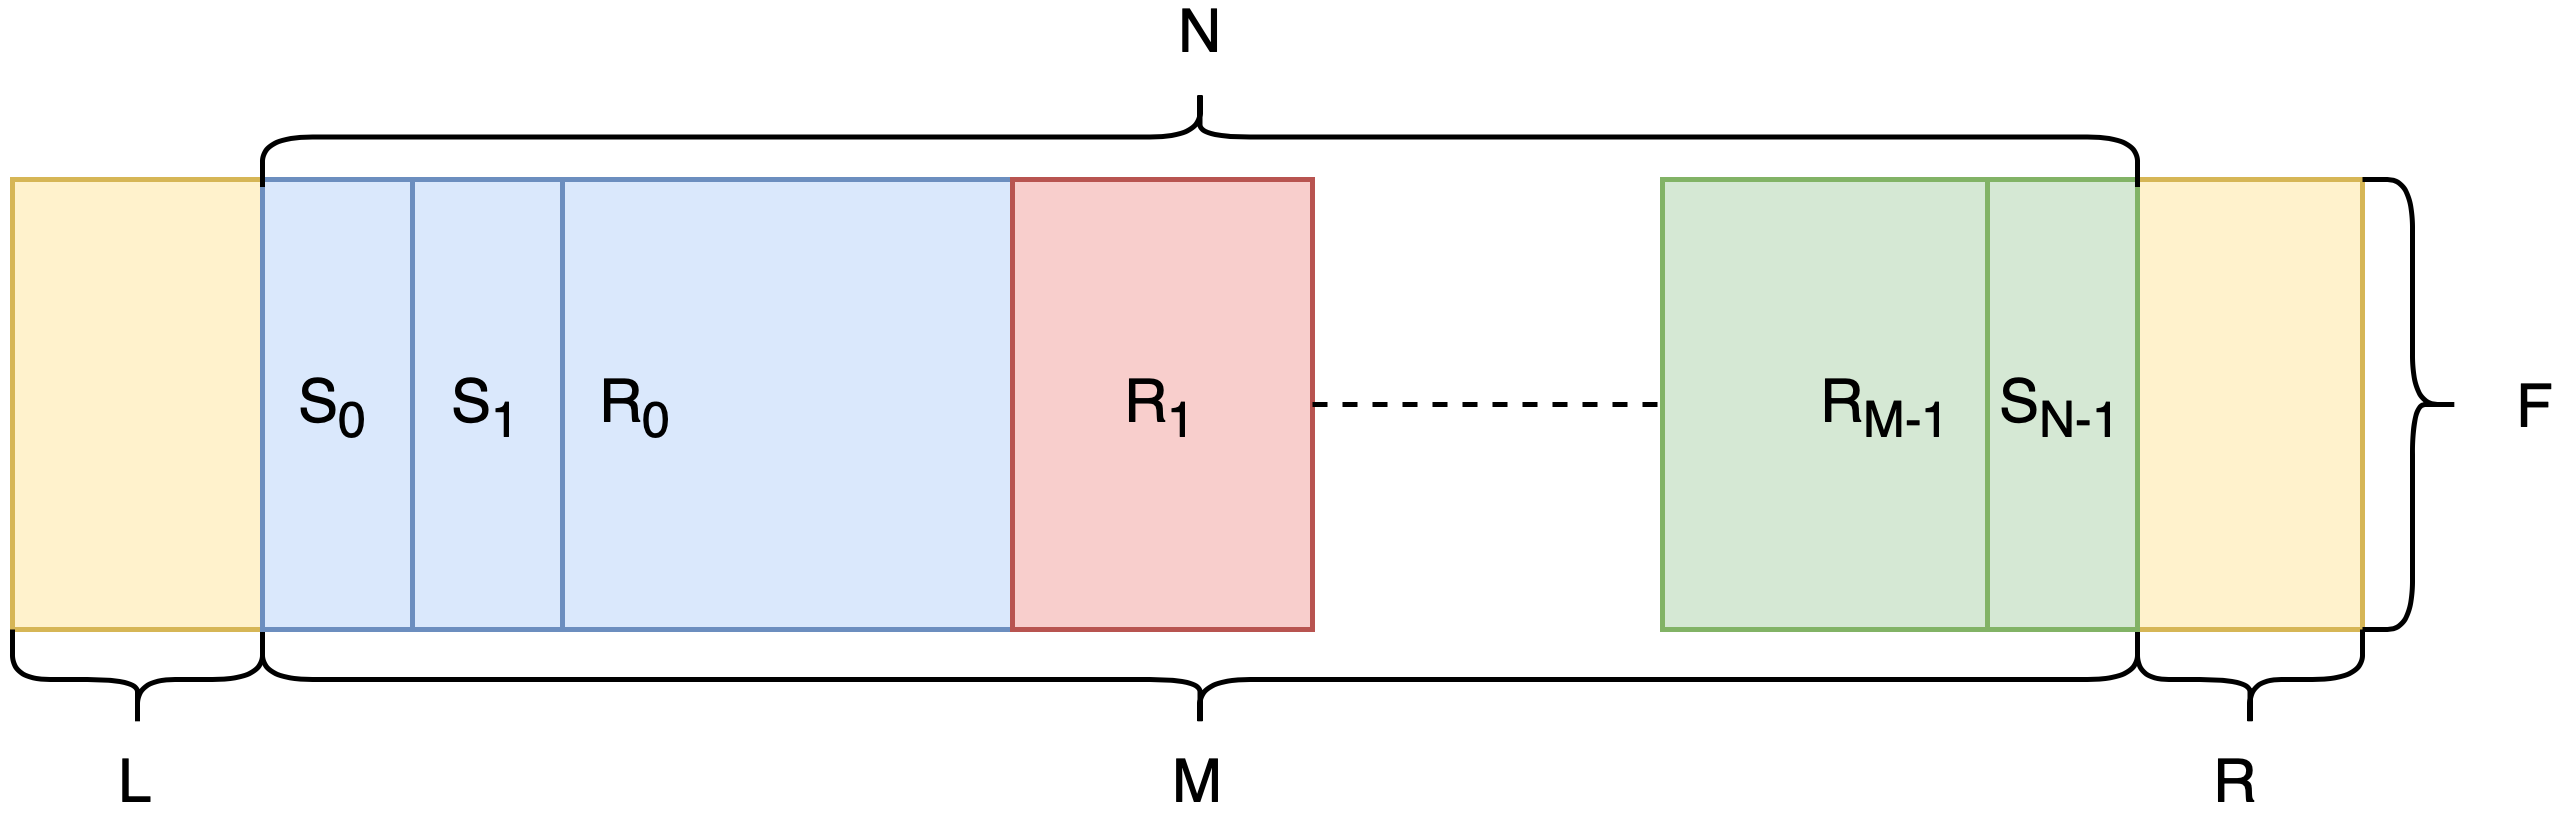
\includegraphics[scale=.125]{dataset_arrangement.png}}
\caption{Uspořádání dat v NumpyDatasetu}
\label{fig}
\end{figure}

kde písmenem $ S $ jsou označeny jednotlivé vzorky. $ R $ označuje jednotlivé nahrávky, které mohou mít různou délku. Písmeno $ N $ udává počet vzorků a $ M $ počet uložených nahrávek. $ L $ a $ R $ značí velikost pravého a levého okraje. Písmeno $ F $ odpovídá počtu příznaků pro jeden vzorek.

Z třídy NumpyDataset dědí třídy NumpyFrameDataset a NumpySampleDataset, které se liší v implementaci metod \_\_len\_\_ a \_\_getitem\_\_. Metoda \_\_len\_\_ při zavolání vrací délku datové sady, která u třídy NumpyFrameDataset odpovídá počtu vzorků a u třídy NumpySampleDataset odpovídá počtu nahrávek. Metoda \_\_getitem\_\_ vrací jeden vzorek z Datasetu, u třídy NumpyFrameDataset vrací metoda jeden vzorek a třídy NumpySampleDataset vrací jednu nahrávku. Třída NumpyDataset je tímto způsobem rozdělena. Důvodem pro rozdělení je, že při načítání dat pro validaci můžeme pomocí třídy NumpySampleDataset spočítat přesnost na celou nahrávku. Naopak při trénování je potřeba načítat vzorky po dávkách, které mají fixní délku na rozdíl od nahrávek, u kterých se délka mění. Vzorky se při trénování často míchají a to je také důvod, proč je lepší mít třídu rozdělenou.

\begin{figure}[h]
\centerline{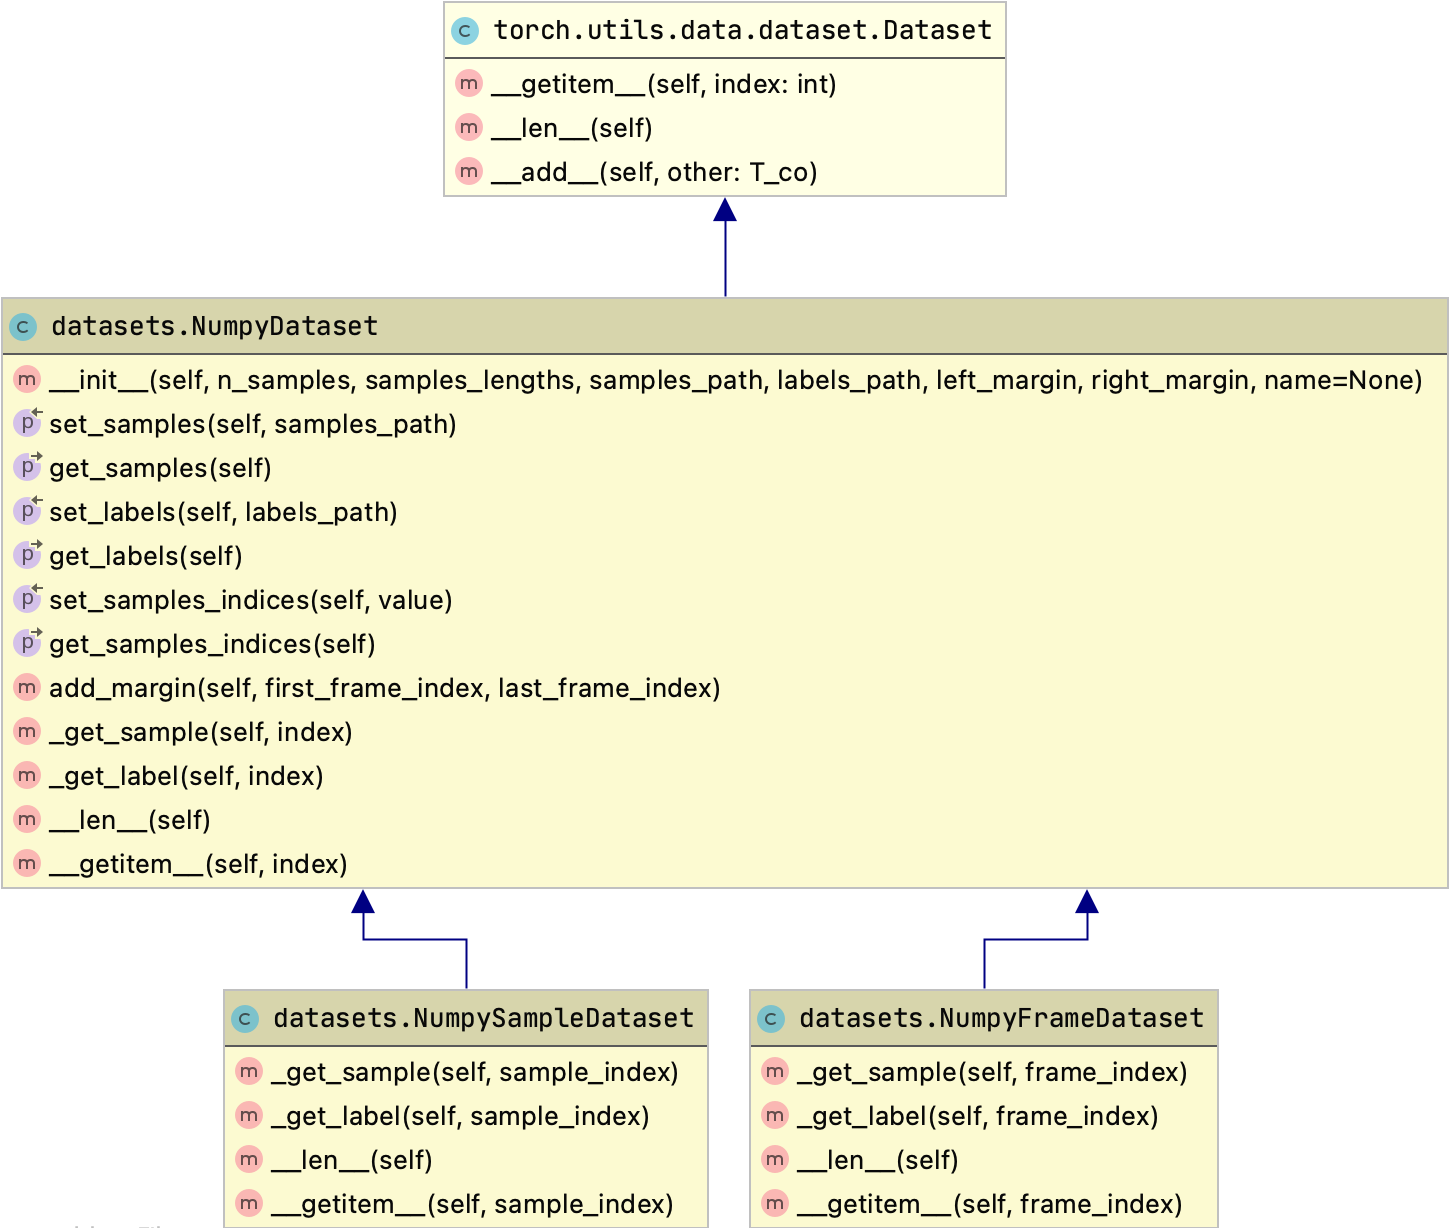
\includegraphics[scale=.2]{datasets.png}}
\caption{Třídy NumpyDataset}
\label{fig}
\end{figure}

Ke vzorkům jsou při výběru přidávány vzorky z okolí pro větší zachycení kontextu nahrávky. Počet vzorků z okolí je načítán na základě velikosti pravého a levého okraje. Vybrané vzorky jsou před vrácením zploštěny. Proces výběru vzorku je znázorněn na následujícím diagramu:

\begin{figure}[h]
\centerline{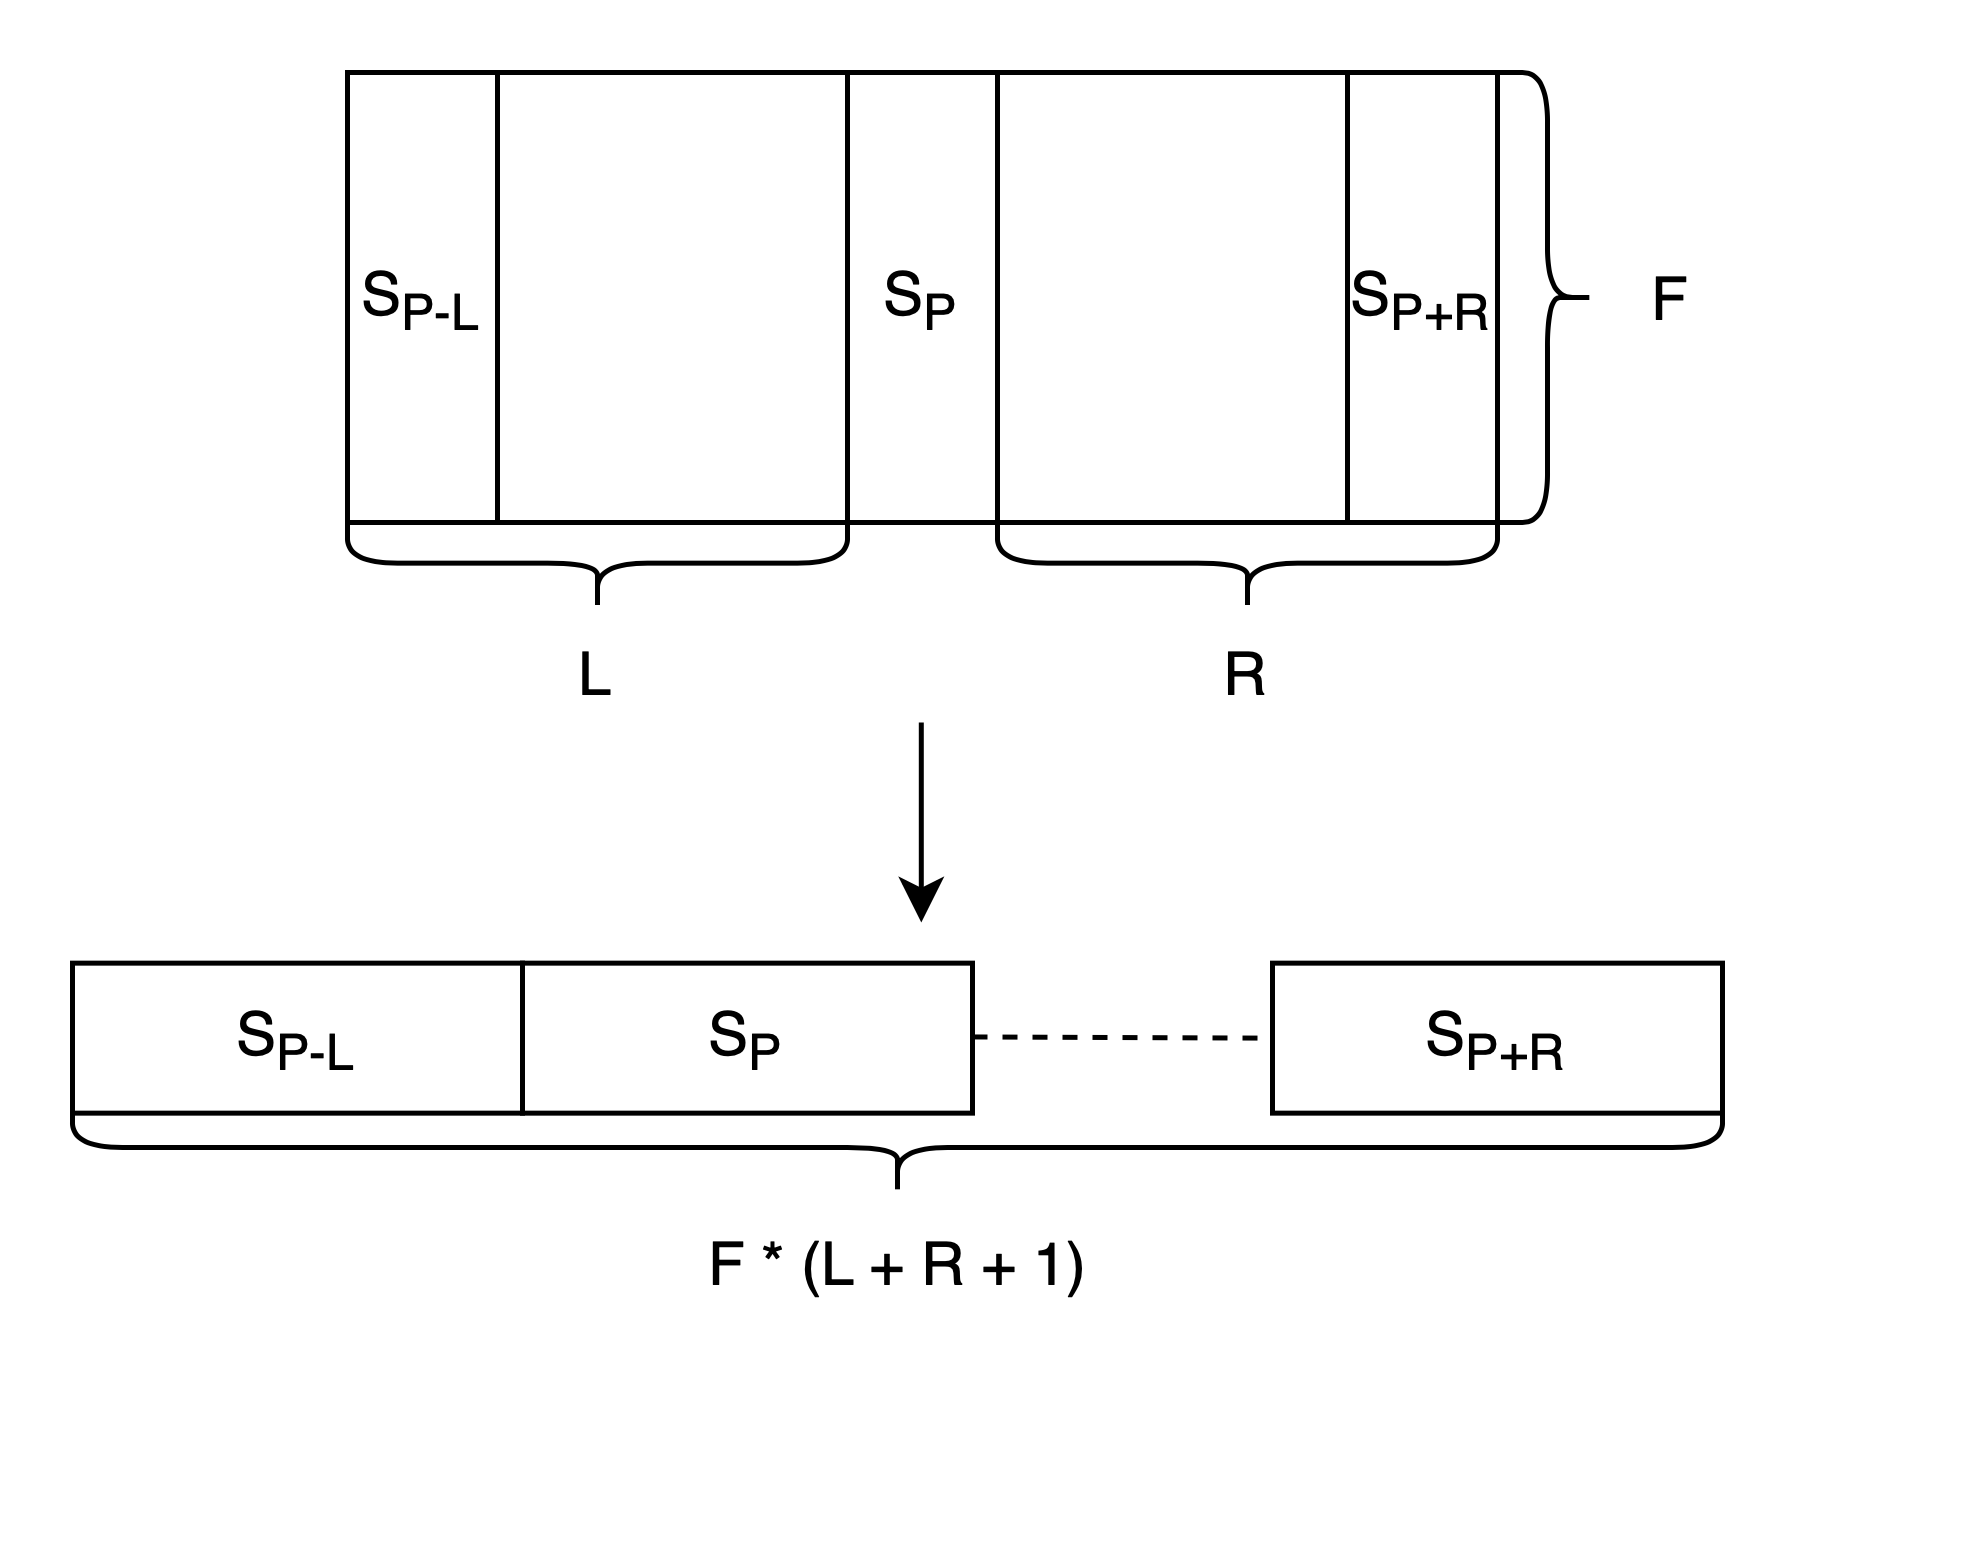
\includegraphics[scale=.125]{sample_selection.png}}
\caption{Výběr vzorku}
\label{fig}
\end{figure}

kde vybraný vzorek má označení $ S $ a krajní vzorky mají označení $ S_{P-L} $ a $ S_{P+R} $. Písmeno $ F $ označuje počet příznaků pro jeden vzorek. Značky $ L $ a $ P $ odpovídají délkám levého a pravého okraje. Výsledný zploštělí obrázek má délku odpovídající $ F * (L + R + 1) $.

\section{Vytvoření neuronové sítě}
Pro vytvoření neuronové sítě byl zvolen framework PyTorch, který je vyvíjen společností Facebook. Dále bylo možné použít framework TensorFlow, který je vyvíjen společností Google. Oba mají velice dobré dokumentace a rozsáhlou komunitu programátorů. Sestavení modelu v TensorFlow je jednoduché. Je možné společně s ním použít framework Keras, který následuje syntax knihovny pro strojové učení scikit-learn. Vytvoření neuronové sítě za pomocí frameworku Keras je velice jednoduché, nicméně neposkytuje tak velkou flexibilitu jako framework PyTorch, kde si kód pro učení, validaci a vyhodnocení může programátor jednoduše napsat sám podle své potřeby. 

Pro vytvoření modelu byl použit objekt Sequential balíčku torch.nn. Model lze inicializovat několika způsoby. Jedním ze způsobů je předáním objektu tuple. Jednotlivé prvky tuplu musí být tvořeny vrstvami modelu, které lze importovat z balíčku torch.nn. Model byl tvořen lineárními vrstvami nn.Linear, které jako vstup berou velikost vstupní vrstvy a velikost vrstvy výstupní. Mezi lineární vrstvy byly umístěny funkce ReLU, který vstupní parametr nemají.

\begin{figure}[htbp]
\centerline{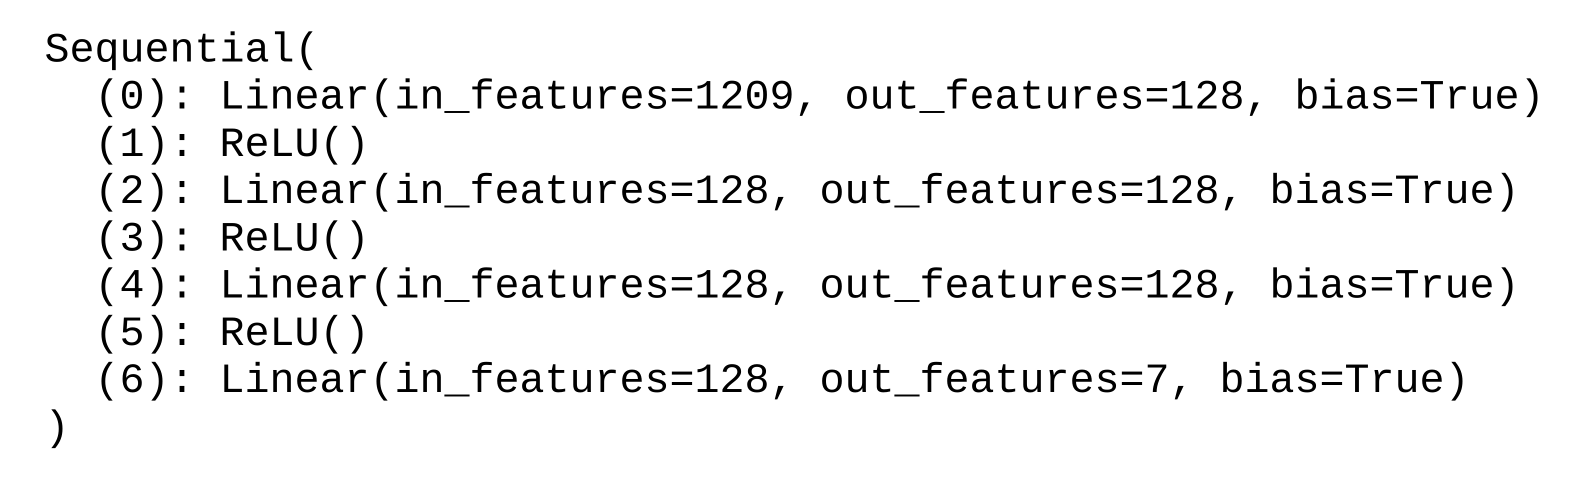
\includegraphics[scale=.25]{model_architecture.png}}
\caption{Ukázka výpisu architektury modelu}
\label{fig}
\end{figure}

Model Sequential byl rozšířen o metodu fit, která se podobá metodě fit používané ve frameworku scikit-learn pro strojové učení. Mezi své parametry bere zdroje dat, které můžou být typu DataLoader nebo Dataset. Dále je pro trénování potřeba předat kriteriální funkci a optimizer. Metoda byla navržena tak, aby bylo možné specifikovat zařízení, na kterém bude trénování probíhat, proto se předává také parametr device. Je možné při trénování na příklad přesunout data s modelem na grafickou kartu pomocí platformy cuda a tím urychlit rychlost trénování. Posledním předaným parametrem je počet epoch, během kterých se má model trénovat.

Byly přidány také metody \_train a \_eval. Metoda train má za úkol trénování modelu. Jako své parametry přebírá trénovací načítače, optimizer, kritérium a zařízení. Model musí být před trénováním nastaven do trénovacího režimu pomocí metody train, která patří modelu nn.Sequential.
Při trénování se načítají data po dávkách z trénovacího načítače a jsou načítány vzorky a štítky. Nejdříve jsou data poslány na zařízení. Dále vynulován gradient optimiteru. Proveden dopředný průchod zavoláním funkce \_\_call\_\_ modelu. Pomocí kritéria je spočítána ztráta modelu, na kterou je zavolána metoda backward, která provede zpětnou propagaci. Při dopředném průchodu je sestavován výpočetní graf, takže si pamatuje cestu zpět. Pomocí metody step optimizeru jsou parametry modelu upraveny. Trénování probíhá, dokud trénovací načítač vrací data pro trénovaní. Při trénování je počítána běžící ztráta, z které lze spočítat průměrnou ztrátu na jednu datovou dávku a po ukončení jednohé epochy trénování i průměrnou ztrátu pro celou trénovací sadu. Dále je počítána přesnost, kdy jsou počítány správně přiřazené vzorky a na konci epochy je z nich spočítána přesnost učení pro danou epochu.

Metoda \_eval se liší od metody \_train hlavně tím, že je na začátku model přepnut do validačního režimu pomocí metody eval. Dále je trénování prováděno v části obsluhované kontextovým manažerem torch.no\_grad, který zajišťuje, že se váhy modelu při validaci nemění. Při trénování byl místo objektu Dataloader používán objekt Dataset, jelikož byla data načítána po jednotlivých nahrávkách. Měla různou délku, a tak nebylo možné použít objekt typu Dataloader. Při trénování byla data před načtením zamíchána, takže nebylo možné určit, do které nahrávky patří. Nicméně při validaci nezáleží na tom, jestli se data před vstupem zamíchají, jelikož nejsou upravovány parametry modelu. Při načítání dat po nahrávkách lze zjistit nejen přesnost předpovědi jednoho vzorku, ale také přesnost předpovědi jedné nahrávky. Pro zjištění přesnosti pro jednu nahrávku byl zjištěna průměrně předpovězená třída. Během validace byly kromě přesnosti a ztráty zaznamenávána matice záměn, kdy byla hodnota ve sloupci se správnou třídou v řádku pro předpovězenou třídu zvýšena hodnota o jedna.

\section{Trénování}
Trénování modelu obstarává objekt Trainer. Při inicializaci je mu předán model, trénovací, testovací a validační data. Objekt má definovanou metodu \_\_call\_\_, jejíž parametry jsou velikost dávky, míra učení, weight decay, počet epoch a název složky kam se mají uložit výsledky trénování. Při zavolí metody je spuštěno logování, které se ukládá do složky s výsledky. Do logovacího souboru se ukládají informace o trénování: zvolené hyperparamtry, výpis modelu a stav trénování. V případě, že nastane chyba při trénování, tak je zaznamenána do logovací souboru, kde je možné si ji přečíst a chybu před dalším trénování opravit. Hlavní funkce, kterou metoda volá je metoda fit modelu.

Metoda fit volá v hlavním cyklu metoda \_train pro trénovací datovou sadu a metodu \_eval pro validační a testovací sady. Počet iterací hlavního cyklu je rovek počtu epoch trénování. Metada fit dále vypisuje do příkazové řádky informace o trénování do přehledného výpisu. Pro každou datovou sadu je vypsána přesnost na jednotlivých vzorcích a ztráta. U validačních a testovacích sad je navíc vypisována přesnost dosažená na celých záznamech. Informace o trénování jsou kromě vypisování také ukládány do datové struktury, která si zaznamenává historii jednotlivých hodnot při trénování. Metoda vrací historii trénování a matici záměn pro poslední epochu trénování.

\begin{figure}[htbp]
\centerline{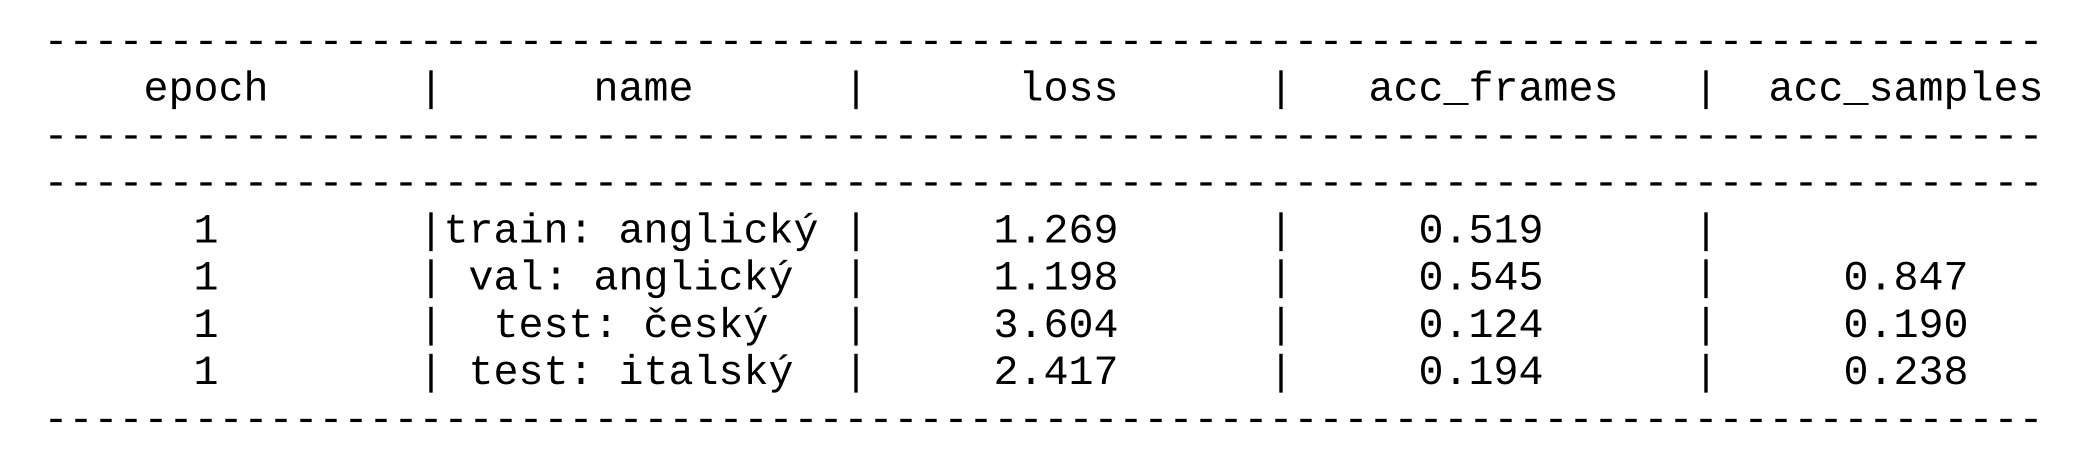
\includegraphics[scale=.215]{train_log.png}}
\caption{Přehledný výpis trénování}
\label{fig}
\end{figure}

Poslední činnost, kterou objekt Trainer vykoná je uložení dat. Při ukládání je do složky s výsledky uložen natrénovaný model pomocí funkce torch.save a výsledky trénování. Mezi výsledky trénování jsou uloženy grafy ztráty a přesnosti. Grafy zobrazující přesnost jsou rozděleny na grafy, které ukazují přesnost pro vzorek a přesnost pro nahrávku. Grafy jsou vytvořené pomocí knihovny matplotlib a její funkce plot. Pro validační a testovací sady jsou uloženy matice záměn, kterou jsou vykresleny pomocí knihovny seaborn a její funkce heatmap. Grafy jsou uloženy jako obrázky ve formátu PNG s rozlišením 200 DPI do složky s výsledky.

$$ acc = \frac{\sum_{c}^{C}{l_c}}{\sum_{i}^{N}{l_i}}  $$ 

$$ p_r = \frac{\sum_{i}^{N}{p_i}}{N} $$

$$ c_s = max(p_s) $$


\chapter{Závěr}

\nocite{*}
\printbibliography[title={Použitá literatura}] % sazba seznamu citací
\addcontentsline{toc}{chapter}{Použitá literatura} % vložení nadpisu do obsahu

\end{document}
